\section{Background}
\label{sec:background}

This thesis introduces two ideas within software engineering which intersect at the need for developer focused tools for software accessibility and the comprehension of the UI screen to facilitate advanced accessibility improvement techniques. To gain a deeper understanding of this intersected research area, it is important to understand the motivation behind each research area and how they benefit each other. 

\subsection{Software Accessibility}

Research in software accessibility relies on the knowledge of various demographics of the disabled community. Most research is focused on solving a problem within a single population of disabled people, for example, a study could test to see if Android applications are accessible to Motor-impaired users \cite{9}, while another could develop a tool to label UI elements in order to help screen readers read out UI elements to visually impaired people \cite{17}. This section will go through how people with different disabilities use touch screen devices. Table \ref{tab:guidelines} lists a series of accessibility guidelines mentioned in previous work as well as the affected user demographic.



\begin{table}[h]
	\footnotesize
	\vspace{-0.0em}
	\caption{Accessibility guidelines extracted from our systematic literature review of accessibility guidelines -- includes recent research and Google's~\cite{GoogleAccess} and Apple's~\cite{AppleAccess} accessibility guidelines. (LV = low vision users, DHH = deaf and hard of hearing users)}
	\vspace{-1em}
	\begin{tabular}{>{\centering\arraybackslash}p{2in}|>{\centering\arraybackslash}p{1.8in}|>{\centering\arraybackslash}p{.82in}|>{\centering\arraybackslash}p{.82in}}
	
		\textbf{Accessibility Guideline} & \textbf{Primary Affected User Demographic} & \textbf{Guideline Source}  & \textbf{Previous Implementation} \\
		\hline
		Visual Touch Target Size & \footnotesize {Motor, LV} & \cite{Kong21, Parhi06} &  \\ 
		\rowcolor{gray!30!} Touch Target Size & \footnotesize {Motor, LV} & \cite{AppleAccess, GoogleAccess, HarvardAccess, WebGuide, Nunes15, Calvo16, Alshayban20, Abascal11, Kane11, Kong21} & X \\ 
		Persistent Element Location & \footnotesize {Motor} &\cite{AppleAccess, HarvardAccess, WebGuide, GoogleAccess} &   \\
		\rowcolor{gray!30!} Clickable Span & \footnotesize {Motor, LV} & \cite{Alshayban20} & X \\
		Duplicate Clickable Bounds & \footnotesize {Motor} & \cite{Alshayban20} & X \\
		\rowcolor{gray!30!} Editable Item Descriptions & \footnotesize {LV} & \cite{Alshayban20, Eler18} & X \\
		Expanding Section Closure & \footnotesize {Motor, LV} & \cite{AppleAccess, GoogleAccess, HarvardAccess, WebGuide} &   \\
		\rowcolor{gray!30!} Non-Native Elements & \footnotesize {Motor, LV} & \cite{GoogleAccess, Calvo16}& X \\
		Motion Activation & \footnotesize {Motor, LV} & \cite{AppleAccess, GoogleAccess, HarvardAccess} &  \\
		\rowcolor{gray!30!} Labeled Elements & \footnotesize {Visual, DHH} & \cite{Alshayban20, FlrezAristizbal19, Li21, Eler18} & X \\
		Screen Captioning & \footnotesize {LV, DHH} & \cite{AppleAccess, GoogleAccess, HarvardAccess, WebGuide, ADAWeb, AccessGov, Ross18, Li21, Pavel20, Kane11}& X \\
		\rowcolor{gray!30!}Keyboard Navigation & \footnotesize {Motor, LV} & \cite{ADAWeb, AccessGov, FlrezAristizbal19, Li21, Chiou21} & X \\
		Traversal Order & \footnotesize {Motor} & \cite{AccessGov, Alshayban20, FlrezAristizbal19} & X \\
		\rowcolor{gray!30!}Adjacent Visual Icon Distance & \footnotesize {Motor} & \cite{AppleAccess, GoogleAccess, WebGuide, Yan19, Abascal11, Nunes15} &  X \\
		
		 Proper Information Organization & \footnotesize {Motor, LV} & \cite{Calvo16} & X \\
		\rowcolor{gray!30!} Facial Recognition & \footnotesize {Motor} & \cite{Calvo16, Astler11} & X \\
		 Single Tap Navigation & \footnotesize {Motor} & \cite{AppleAccess, GoogleAccess, HarvardAccess, WebGuide, FlrezAristizbal19, Milne18} &  \\
		\rowcolor{gray!30!} Poor form design/instructions & \footnotesize {Motor, LV} & \cite{ADAWeb, AccessGov} &  
		\end{tabular}
\vspace{-1em}
	\label{tab:guidelines}
\end{table}



\noindent \textbf{\textit{Visually Impaired Users}}

Visually impaired users use screen readers about 90.5\% of the time \cite{17}. Low vision (LV) users, or users who can see, but not to the extent that legally blind people can, do not always depend on screen readers. They depend on being able to see contrast in UI design and fonts, making it so that elements and text on the screen are clearly visible and large enough for them to read \cite{31}. LV users do not only depend on being able to see and navigate the screen, various keystrokes and actions are required in order to interact with touch screen devices. 

\begin{figure}
    \centering
    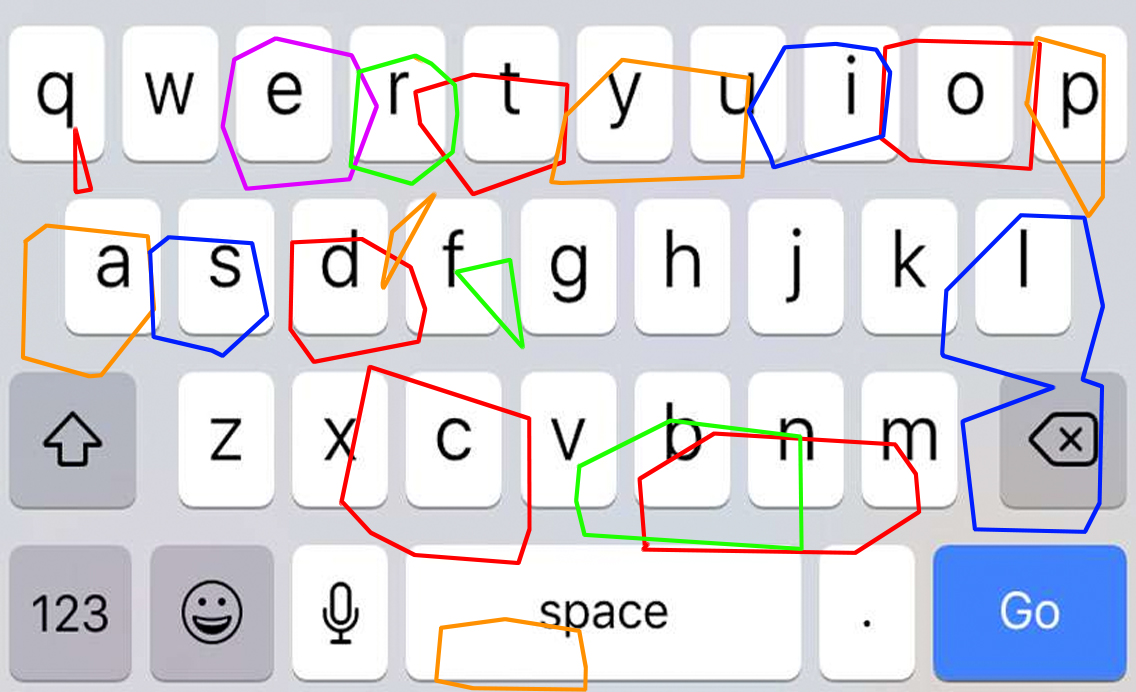
\includegraphics[width=0.5\textwidth]{imgs/hits.jpg}
    \caption{Polygons representing clusters of hit points for LV users \cite{4}}
    \label{fig:HitPoint}
\end{figure}

An example of this is shown in Figure \ref{fig:HitPoint}. LV users have difficulty seeing the screen and resort to guessing where their taps land. The image shows clustered taps in an attempt to type out sentences on a touch device. It is clear that LV users are not properly able to tap where they intend to. Speech to text \cite{25,26} or braille inputs are a way for LV users to effectively input information into the device \cite{33}. Keystrokes are identified by gesture recognizers built within touch screen devices \cite{12}. These recognizers are built with the able-bodied user in mind, so companies like Apple and Google allow users to modify the sensitivity and duration of the touch inputs \cite{12,25,26}. These accessibility measures help LV users use their devices more efficiently.\\ 

\noindent \textbf{\textit{Deaf and Hard of Hearing Users}}
 
Deaf and Hard of Hearing (DHH) users, unlike LV users, are comfortably able to physically use their touchscreen devices. DHH users need live captioning or American-Sign-Language (ASL) interpretations of any audio outputted by the device \cite{5}. There are currently tools that provide live captioning \cite{34} and research that is being done in converting audio to ASL depictions for users \cite{35}. DHH users also rely on text-to-speech or limited verbal communication to provide audio inputs into their devices \cite{36}.\\

\noindent \textbf{\textit{Motor-impaired Users}}
\begin{figure}[h]
    \centering
    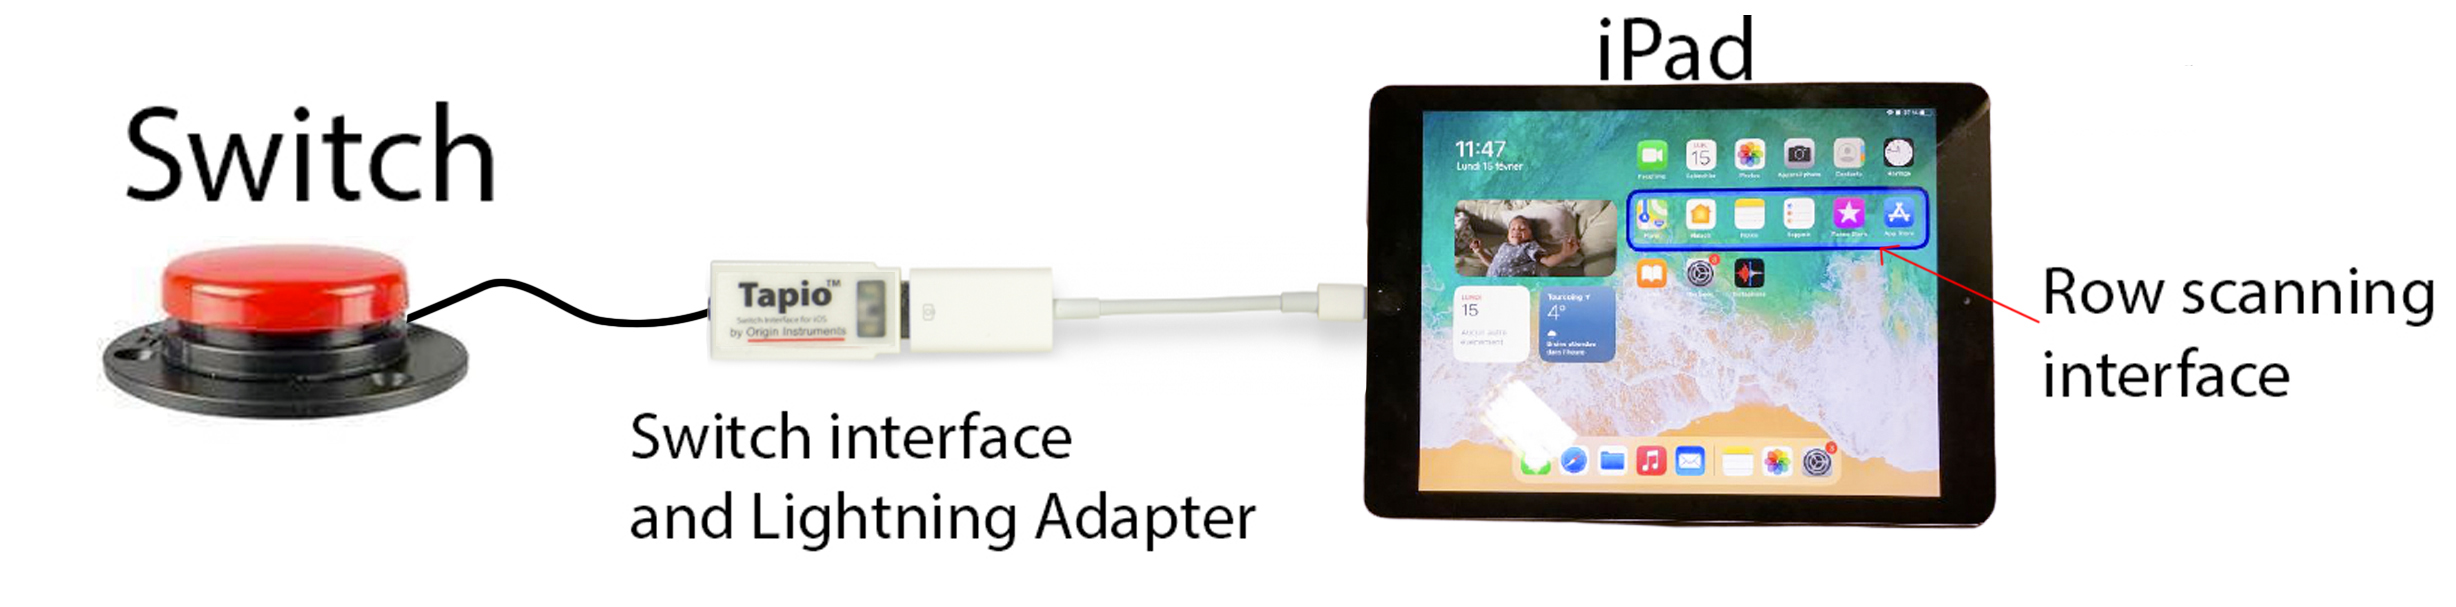
\includegraphics[width=0.6\textwidth]{imgs/switchInterface.jpg}
    \caption{Switch Interface}
    \label{fig:SwitchInterface}
\end{figure}

Motor-impaired users use devices in two main ways: Switch input and touch input \cite{2}. Switch based input uses an external hardware input device. Switches are common in users with limited to no motor control who still retain their cognitive functions \cite{2}. Current touch devices offer scanning methods that scan a curser across the screen and highlights them as they pass \cite{25,26}. The users then can click the switch and select the application that is highlighted and continue using the device. An example of this switch interface is shows in Figure \ref{fig:SwitchInterface}. The most commonly used switch is a single input switch, which is then connected to an adapter to create signals for the device, and then to the device, in this case, an iPad. The iPad then can scan and highlight rows and columns for the user to tap on the switch and select. This gets very tedious as average words per minute typed using tradition scanning based techniques is 3, which is significantly lower than the average normal users, which is, 39 \cite{37}. The other form of input, touch input, is the same as a normal user, but motor-impaired users generally have a tremor or lack of speed in gestures made on the screen. Slightly motor-impaired users also find themselves using voice commands to navigate applications and send messages since keyboards can be frustrating to use with smaller keys \cite{2}. Work has been done to improve gesture recognition. Google and Apple offer sensitivity and touch settings that allow users to better physically interact with their devices \cite{12,25,26}.\\ 

\noindent \textbf{\textit{Neurodivergent and Cognitively Impaired Users}}

This demographic of users is primarily classified as individuals with cerebral differences such as Attention-deficit/hyperactivity disorder (ADHD), Autism Spectrum Disorder (ASD), dyslexia, and memory loss. It is estimated that 7\% of the population identifies as neurodivergent-encompassing cognitive and learning disabilities \cite{48}. These users, unlike the users presented previously, are severely underrepresented in design of the web. The Web Content Accessibility Guidelines (WCAG) \cite{49} requires accessibility measures for LV, DHH, and motor-impaired users, but does not require the implementation of neurodivergent supporting guidelines. Software and tools that neurodivergent users rely on tend to be low-sensory to avoid sensory overload. Users who are distracted easily or have highly receptive cognitive functionality tend to need software where there is a clear focal point to each functionality in the application without the need of unnecessary animations and sounds \cite{50}. The current set of applications provides many complex avenues of accessing information, but can be challenging to neurodivergent users. An application like Twitter, for example, has an abundance of scrolling animation and task bars that can be used to navigate the app. The animations, videos playing, and options of navigation can overload users since there is no focal point to the screen and what the user should be looking at. 

\subsection{Developer Tools for Accessibility}

The current landscape of developer tools is limited. Studies have shown that current developers do not utilize tools or ignore them because they introduce warnings, some of which are completely wrong \cite{9}. In this survey we found very few developer-specific tools, but found many studies that looked at software guidelines for developers. Guidelines are set for developers on all platforms to make their websites and applications more accessible \cite{25,26,38,18}. GUI guidelines require developers to abide by certain standards and practices in order to help disabled users navigate and use the application as intended. Guidelines specify certain requirements for elements such as size, placement, and color contrast to help users see tap and see them easier \cite{25,26}.


\subsection{UI Understanding}

Much of the research in accessible GUI analysis has been done in UI enhancement and UI comprehension for use in accessibility studies, hence it is important to understand the current state of UI comprehension techniques. Accessibility based UI augmentation and comprehension is only as good as the current techniques in the field. 

Wu et al. \cite{41} worked on a screen parser that is able to predict relationships within elements on the screen. They did this by training a Faster-RCNN using thousands of both IOS and Android screenshots. Then they  determined node correspondence and extracted hierarchical correspondence for each of the elements. Then they grouped the elements together into groups that were under a certain category. So interactive elements were one group while background and images would have been another group \cite{41}. This work was done to better understand the relation between elements on the screen, but can also be used to label and identify screen elements and traverse them in a better order for users with disabilities. This approach was expensive and the UIElement detector they used was observed to slow other processes down.

Most accessibility software tools have been related to testing where researchers tend to find accessibility guideline violations. Moran et al. \cite{42} worked to create an automated GUI checker that checks to see if GUIs were made to their intended design \cite{42}. They then used a GUI comprehension technique and a set of design violations to work on a detector that would detect design violations. It gave promising results that correctly detected design violations in Android apps. This visual GUI testing (VGT) is a great way to start testing for more accessible GUIs. This testing method, however, does not allow GUI boxes to overlap and requires a straightforward GUI. This can hinder GUI mockups and novice developers from being able to test for violations. 

Like the project by Moran et al \cite{42}, UIBert by Google \cite{43} works to identify and comprehend screen elements. It works by taking in UIs and parsing it to identify all of the elements. It then uses that information to predict which type of app it is. It classifies the icons and then uses those generalized icon predictions to make an app prediction. This is a way for UI comprehension to be useful for screen readers or voice assistants to be able to access a certain type of app, e.g. games or music \cite{43}.  

It is really important to understand GUIs when looking to help developers make more accessible software because most techniques from GUI comprehension are used to label and modify GUIs to make applications more accessible, so by looking at the current research in this field, we can see how GUI accessibility is dependent on advancements in GUI comprehension. 



























